% Chapter 2

\chapter{Models for random simplicial complexes} % Main chapter title

\label{Chapter2} % For referencing the chapter elsewhere, use \ref{Chapter1} 

\lhead{Chapter 2. \emph{Random models for the curve complex}} % This is for the header on each page - perhaps a shortened title

%----------------------------------------------------------------------------------------

The use of the probabilistic method in discrete mathematics has become a prominent ideas in the area in recent times. It has been used to provide existence proofs where objects have certain desirable properties and it's not always easy to construct explicit examples. This has been just the beginning of the use of probabilistic tools in a deterministic context.

Leaving aside all the applied problems, probability theory can help us to understand the ubiquity of certain mathematical phenomena. For example, \textit{many} simplicial complexes and posets which arise from combinatorial constructions are homotopy equivalent to a wedge of spheres. There's also a well-known theorem that states that hiperbolicity is \textit{quite common} in random groups, meaning that even under different measures, almost every group is hyperbolic.

We are interested in giving formal meaning to expressions like \textit{"quite common"} or \textit{"many"}. In particular we're interested in studying \textit{"typical"} topological properties of random simplicial complexes, for a great survey in this subject we can refer to \cite[M. Khale]{surveyStochastic}. The idea is to provide tractable toy models using the combinatorial language that was obtained from the translation of rigidity phenomena. In chapter one we precisely settle the base that will allow us to model the curve complex or the curve graph associated to any given surface. In this chapter we'll will review the most popular and feasible models and explain how to choose the parameters to couple the model into the desire framework. We'll also review rigid expansions in a probabilistic perspective.

Familiarity with basic concepts in probability theory such as probability spaces, random variables, and basic theorems will be assumed.

\section{The Radó graph}

The curve graph satisfy the following properties:

\begin{enumerate}
\item Infinite countable number of vertices
\item Connected.
\item Locally infinite.
\item Clique number $3g-3+m$.
\item Infinite diameter.
\end{enumerate}

The first property might tell us to directly look for a model which consider an infinite number of vertex, it's well know by \cite[Erdös, Rényi]{RadoUnique} that every infinite random graph is isomorphic to the Radó graph. The Radó graph is a countably infinite graph that can be constructed (with probability one) by deciding independently for each pair of its vertices whether to connect them by an edge or not.

A construction for this graph can be done by using binary numbers. To do this we identify the vertices of the graph with the natural numbers, and then every edge appears between vertices $x$ and $y$ in the graph (assuming $x < y$) whenever the $x$-th bit of the binary representation of $y$ is nonzero. This means that all odd-numbered vertices will be neighbors of vertex 0. The larger neighbors of vertex 1 are all vertices with numbers congruent to 2 or 3 mod 4.

This graph satisfy that every finite or countably infinite graph is an induced subgraph of it. Even more, any graph of this type can be found as an induced subgraph by an algorithm (more precisely a greedy algorithm) that builds up the subgraph one vertex at a time. From here we can see that if we start from a surface $S$ of finite genus then, because of the restriction of the clique number in $C(S)$, it's not possible that the Rado graph is embeded into $C(S)$. Not only that, it turns out that the converse is also valid, there's the following result by \cite{} (Bering and Gaster).

\begin{theorem}
The random graph embeds into the curve graph $C(S)$ of a surface $S$ if and only if $S$ has infinite genus.
\end{theorem}

So, if we want to study the curve graph of a surface of finite genus through the Rado graph, we have to think it as a subgraph of it. If we take uniformly random vertices of the Rado graph then



At this point we have that we will not be able to build the curve graph by an uniform selection of vertices. The problem here is that we want to sample a space with very specific clique number (notice that this is the only property of the curve complex listed above which actually depends on the genus of the surface). But this isn't new, a common problem is that some times we want to sample in spaces with certain properties. 

An example of this is when we want to ensure that the random graph doesn't have cycles \cite{Alcazar15})( in this case it's implied that the clique number is 2). If we don't do things carefully we'll lose the i.i.d properties that we are looking for. A discrete MCMC algorithm can be used to sample uniformly random trees of size $n$, for example with the \texttt{generate algorithm} we can produce a maximal tree of any not directed graph with $n$ vertices taken uniformly among all the possibles ones. The justification of this last fact can be found in \cite{Broder89}. A summarize of this method can be find in the appendix.

Even if we can provide an analog of the generate algorithm which ensure any other fixed clique number, the idea is to study rigid expansions in a simpler probabilistic approach. So another good idea will be to use a finite proposal for random graphs such as the Erdös-Rényi model, and then make asymptotic arguments. The simplicity of the model had made it very popular in stochastic topology; it consists in considering $n$ vertices and then each of the possible edges appear with probability $p$ (usually we want to take $p=p(n)$). With this prospect in mind we will keep the idea of having a uniform simple model.

\begin{defini}
We will denote by $\G(n,p)$ to the probability space formed by all the graphs of $n$ vertices and probability measure 
$$ \P(G\in \G(n,p)) = p^{k} (1-p)^{\binom{n}{2}-k} $$
where $k$ is the number of edges in $G$, the $\sigma$-algebra is given by the power set.
\end{defini}

It's usual to find a variation of the model where $m$ is rather consider as a parameter of the model. We pick randomly $k$ edges among the $\binom{n}{2}$ possible. 

Notice that we can also think this model like $\binom{n}{2}$ Bernoulli random variables identically and independently distributed with parameter $p$ that represents the edges. Using what we know about the Binomial r.v. we can immediately get some properties of the degree of a given vertex $v$. 

\begin{itemize}
\item The probability that a given vertex $v$ has degree $k$ is given by
$$b(k; n-1,p) = \binom{n-1}{k} \cdot p^{k} \cdot (p-1)^{n-k-1}$$
\item The expected degree is $(n-1)\cdot p$
\item The variance of this degree is $(n-1)\cdot p \cdot (1-p)$
\end{itemize}

We'll keep in mind the degree distribution because, as we'll see in the next chapter, it will be important to keep track of leaves and isolated vertices to do some optimizations in our algorithms.

We can use the Erdös-Rényi model to obtain random simplicial complexes through clique complexes. The clique complex or flag complex $X(G)$, of a graph $G$ is the simplicial complex with all complete subgraphs of $G$ as its faces. The 1-skeleton of $X(G)$ is $G$ itself. $X(G(n, p))$ will be abbreviated by $X(n, p)$ for now on.

\section{Finding the parameters of the model}

In this section we present a recompilation of asymptotic claims for the Erdös-Rényi model for properties that concern the curve complex.

\subsection{Connectivity}
\begin{theorem}
Let $\omega(n)$ be a function that tends to infinity arbitrarily slow as $n$ tends to infinity
\begin{itemize}
\item If $p\geq \frac{log(n)+ \omega(n)}{n}$ then 
$$\lim_{n \to \infty} \P(G \in \G(n,p) \text{ is connected}) = 1$$
\item If $p\leq \frac{log(n)- \omega(n)}{n}$ then
$$\lim_{n \to \infty} \P(G \in \G(n,p) \text{ is disconnected}) = 1$$
\end{itemize}
\end{theorem}
 
 This can be proven by first showing that for a large $n$ almost all graphs consists of a connected graph having $n-k$ effective vertices and $k$ isolated points, the theorem follows from a counting argument. The complete proof can be found in \cite[Erdös-Rényi, 59]{OnRandomGraphs}.
 
 
\subsection{Locally infinity}

We already discuss that $deg(v)$ behaves like a binomial random variable. So we just have to describe $p$ so that a.a.s $deg(v)$ tends to infinite along with $n$. Consider $v\in V(G(n+1,p))$, so:
$$ \P(deg(v)=k) = \binom{n}{k} \cdot p^{k} \cdot (1-p)^{n-k}$$
Let $\epsilon>0$ and $a>0$ be fixed, taking $p=\frac{\epsilon}{n^{a}}$ we have
\begin{center}
\begin{tabular}{ r l }
 $\displaystyle\lim_{n\to \infty } \P(deg(v)=k) =$ & $\displaystyle\lim_{n\to \infty} \binom{n}{k} \cdot \left( \frac{\epsilon}{n^a} \right)^k \cdot \left( 1-\frac{\epsilon}{n^a}\right)^{n-k}$ \\
 $\sim$ &  $\displaystyle\lim_{n\to \infty} \frac{n^k}{k!}\cdot  \frac{\left(\frac{\epsilon}{n^a}\right)^k} {\left(\frac{n^a - \epsilon}{n^a}\right)^k} \cdot \left(1-\frac{\epsilon}{n^a}\right)^{n} $\\
$=$ &  $\displaystyle\lim_{n\to \infty} \frac{n^k}{k!}\cdot \left(\frac{\epsilon} {n^a - \epsilon}\right)^k \cdot \left(1-\frac{\epsilon}{n^a}\right)^{n} $\\
\end{tabular}
\end{center}
the last term of this expression have a very interesting asymptotic behavior, when $a=1$ we already know that $\left(1-\frac{\epsilon}{n^a}\right)^{n} \to e^{-\epsilon}$ which actually determine the Poisson approximation of the Binomial random variable. When $a\neq 1$ then we have to do the following analysis
$$\displaystyle\lim_{n\to \infty } \left( 1 - \frac{\epsilon}{n^a}\right)^n = \displaystyle\lim_{n\to \infty} exp\left( ln \left( 1 - \frac{\epsilon}{n^a}\right)^n\right) = \displaystyle\lim_{n\to \infty} exp\left(n \cdot ln \left( 1 - \frac{\epsilon}{n^a}\right)\right)$$
So we need to study $\displaystyle\lim_{n\to \infty} f(n) = \displaystyle\lim_{n\to \infty} n \cdot ln \left( 1 - \frac{\epsilon}{n^a}\right)= \displaystyle\lim_{n\to \infty}\frac{ln \left( 1 - \frac{\epsilon}{n^a}\right)}{\frac{1}{n}}$, using L'ôpital's rule for limits we obtain:
$$\displaystyle\lim_{n\to \infty } f(n) = 
\displaystyle\lim_{n\to \infty } \frac{\frac{1}{\left( 1 - \frac{\epsilon}{n^a}\right)}\cdot (\epsilon a n^{-a-1})}
{-1\cdot n^{-2}} = 
\displaystyle\lim_{n\to \infty } \frac{\frac{n^a}{n^{a} - \epsilon}\cdot (\epsilon a n^{-a-1}) \cdot {n^{2}}}{-1} = 
\displaystyle\lim_{n\to \infty } - \frac{\epsilon a n}{n^{a} - \epsilon} =
\displaystyle\lim_{n\to \infty } - \frac{\epsilon a}{a n^{a-1}}
$$
from here we can see that if $a>1$ then $\displaystyle\lim_{n\to \infty } f(n) = 0$ and if $a<1$  then $\displaystyle\lim_{n\to \infty } f(n) = -\infty$
Notice that $\P(deg(v)=0) = \left(1 - \frac{\epsilon}{n^a} \right)^n$, so:
$$ \displaystyle\lim_{n\to \infty} \P\left(deg(v)=0\right) = \begin{cases} 
\displaystyle\lim_{n\to \infty}e^{f(n)} = 1, & \mbox{if } a>1 \\ 
\displaystyle\lim_{n\to \infty}e^{f(n)} = 0, & \mbox{if } a<1 \end{cases} $$

Another perspective to study the degree of vertices is to consider $X_{k} = X_{k} (G)$, the random variable that describes the number of vertices of degree $k$ in a graph $G$. The following theorem gives a describe this invariant.

\begin{theorem}
Let $\epsilon>0$ be fixed, $\epsilon n^{-3/2} \leq p = p(n) \leq 1 - \epsilon n^{-3/2}$, let $k = k(n)$ be a natural number and set $\lambda_{k} = \lambda_{k}(n) = n\cdot b(k;n - 1,p)$. Then the following assertions hold.

\begin{itemize}
\item If $\lim \lambda_{k}(n) = 0$, then $\lim P(X_{k} = 0) = 1$. 
\item If $\lim \lambda_{k}(n) = \infty$, then $\lim P(X_{k} > t) = 1$
for every fixed $t$.
\item If $0 < \lim\lambda_{k}(n) < \lim \lambda_{k}(n) < \infty$,
then $X_{k}$ has asymptotically Poisson distribution with mean $\lambda_{k}$: 
$$P(X_{k} = r) \sim e^{\lambda_{k}}\cdot \lambda_{k}^{r}/ r!$$
for every fixed $r$.
\end{itemize}
\end{theorem}

The hypothesis on $ p $ appears when we consider a loose upper bound on the expected degree of $ X_ {k} $, using this bound we can directly assert that if $ pn ^ {2} \ to \ infty $ then almost every $ G \ in G (n, p) $ consist of independent edges and isolated vertices. The complete argument of this claim among with the proof of the theorem can be found in \ cite [Bollobás, p.61] {Bollobas}.

If $k$ is a finite fixed number, then the past theorem is saying that when $\lim \lambda_{k}(n) = 0$ then a.a.s there aren't vertices of finite degree. In the second case we obtain that there are as many vertices with degree $k$. And in the third case we can describe explicitly the degree distribution, which concentrate the degree in a finite range arround the mean $\lambda_{k}$. So to fit the model into the context of the curve complex we need to choose $p = p(n)$ so that the first case is satisfied for any fixed $k$ i.e.
$$\lambda_{k} = n \binom{n-1}{k} p^{k} (1-p)^{n-k-1} \to 0$$

\subsection{Clique number}
Let $Y_{r}$ be the random variable that counts the number of $r-$cliques.
$$\E(Y_{r}) = \binom{n}{r} \cdot (1-p^{r})^{n-r} \cdot p^{\binom{r}{2}}  $$
The following theorem describe the conditions to obtain a particular clique number.

\begin{theorem}
Let $r = r(n) = O(n^{1/3})$ and let $p=p(n)$, $0<p<1$, be such that
$$\binom{n}{r} p^{\binom{r}{2}} \to \infty \text{ and } \binom{n}{r+1} p^{\binom{r+1}{2}} \to 0 $$
Then a.e $G_{p}$ has clique number $r$
\end{theorem}
The second condition on $p$ implies that almost no $G_{p}$ contains a $K^{r+1}$ so $cl(G_{p})\leq r$ asymptotically almost surely. The first condition on $p$ is simply that $\E (Y_{r}) \to  \infty$. The idea to proof this theorem is to use the calculations for $\E(Y_{r})$ and a first moment argument will work for the rest of the argument. A full proof can be find in \cite[Bollobás, p.290]{Bollobas}.

We want $r = 3g-3+m$, where $g$ is the genus and $m$ is the number of punctures. $p(n)$ should be taken in a way that the hypothesis in the theorem gets satisfied when we take $r$ to be a constant.

%$$\binom{n}{r} p^{\binom{r}{2}} \sim \frac{n^{r}}{r!} p^{\frac{r(r-1)}{2}} = \lambda (np^{r-1/2})^{r} $$

%where $\lambda$ its a constant and $ \lim_{n \to \infty} \lambda (np^{r/2})^{r+1} = 0  \iff  (np^{r/2}) \to $

%$$\binom{n}{r+1} p^{\binom{r+1}{2}} \sim \frac{n^{r+1}}{(r+1)!} p^{\frac{(r+1)r}{2}} = \lambda (np^{r/2})^{r+1} $$

%where $ \lambda (np^{r/2})^{r+1} \to 0  \iff  (np^{r/2}) \to $


%--------------------------%
%We can checked that if $\epsilon > 0 $ and $n$ is sufficiently large, then $\E(Z_{r})$ is large for all $r$'s between $(\frac{1}{2} + \epsilon)r_{0}(n)$ and $(1 - \epsilon)r_{0}(n)$ and small for all $r$'s outside the range $\{ (\frac{1}{2} - \epsilon)r_{0}(n), (1 + \epsilon)r_{0}(n) \}$



%\begin{theorem}
%Given constants $0 < p < 1$ and $0<\epsilon<\frac{1}{2}$ a.e. random graph in $\G(n,p)$ is such that it has a clique of order $r$ for all $r$ satisfying 
%$(1+\epsilon)log_{b}(n) < r <(2-\epsilon) log_{b}(n)$
%but has no clique of order $r$ if $r < (1-\epsilon)log_{b} (n)$ or if $r<(2+\epsilon)log_{b}(n)$
%\end{theorem}

%There's another point of view which is more popular to study the question for the clique number of a random graph. Matula was the first to notice that for fixed values of $p$ the distribution of the clique number of a random Graph is highly concentrated: almost all $G_{p}$ have about the same clique number. Results asserting this phenomenon were proved by Grimmett and McDiarmid.

%{\color{Blue} Bólobas 290}

%There's a result for the clique number for random graphs in the sense of the Rado Graph}
%--------------------------%


\subsection{Diameter}

The diameter of a graph $G$, denoted by $diam(G)$, is the maximal distance between pairs of vertices of $G$. Thhe following theorem can be found in \cite[Bollobás, p.259]{Bollobas}




This means that if we want to have infinite diameter, we need that $d$ tends to infinity as $n$ does, while the condition $pn/(log\text{ }n)^{3} \to \infty$ is also satisfied i.e.
$$ \frac{(n\cdot\text{log}(n^{2}/c))^{1/d}}{(\text{log n})^{3}} \to \infty$$

  

\begin{theorem}
If $p$ is taken fixed $G(n,p)$ has diameter 2 with high probability 
\end{theorem}

\begin{proof}
Consider the random variable $X_{n}$ which is the number of vertex pairs in a graph in $\G(n,p)$ with no common neighbors. By Markov's inequallity we have that

$$\P(X_{n} \geq 1)\leq \E(X_{n}) = \binom{n}{2} \cdot \P(\text{two vertices doesn't have common neighbors}) = \binom{n}{2} (1-p^{2})^{n-2}$$

which tends to zero as $n\to \infty$
\end{proof}



\section{Uniquely determined vertices}

In the last chapter we settled the background for rigid expansions, with this combinatorial approach we should have the following calculations to study rigidity phenomena.

\begin{itemize}
\item What is the probability that a vertex $v$ is uniquely determined by a set of size $k$? (Event $E_1$)
\item What is the probability that a set of size $k$ generate a rigid expansion? (Event $E_3$)
\end{itemize}

For the first event take a look to the following picture

\begin{figure}[h!]
	\centering
	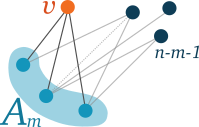
\includegraphics[scale=0.8]{figures/uni.png}
	\caption{Probability of uniquely determined vertices}
\end{figure}

i.e. if $<A> = v$ with $|A| = m$ then there's a edge between $v$ and every vertex in $A$, and none of the $n-m-1$ remaining vertices is also connected to every vertex in $A$, i.e.
$$\P(E_1(m)) = p^{m}(1-p^{m})^{n-m-1}$$

For the second question we have that if $A_k$ does not generate a rigid expansion is because none of the possible subsets of $A_k$ determined uniquely a vertex outside of $A_k$. 

We have that the probability that none of the vertices outside of $A_k$ is uniquely determined by $A_m\subset A_k$ is $\rho_{m,k} = (1 -  \P(E_1(m) )^{n-k}$.

$$\P(A_k \text{generates a rigid expansion}) = 1 -  \Pi_{m=1}^{k} (\rho_{k,m})^{\binom{k}{m}}  $$

Using the \texttt{networkx} library in \texttt{python} we obtained simulations for this phenomena and then compare them with the past calculations, in the next chapter we'll explain a little bit more

\begin{figure}[h!]
	\centering
	\includegraphics[scale=0.5]{figures/fixed-uniq-det.png}
	\caption{Probability of uniquely determined vertex, varying $k$ in $A_k$}
\end{figure}

\begin{figure}[h!]
	\centering
	\includegraphics[scale=0.5]{figures/rig-prob.png}
	\caption{Probability of having a rigid expansion,  varying $k$ in $A_k$}
\end{figure}

We mention in the first chapter the property that 


That's why it's worth to enunciate the following theorem which can be found in \cite[Khale, 16]{Khale}.
\begin{theorem}
Let $k \geq 3$ and $\epsilon > 0$ be fixed. If
$$\left(\frac{(C_{k} + \epsilon \text{log } n} {n} \right) n^{1/k} \leq p \leq \frac{n^{-\epsilon}}{n^{1/(k+1)+\epsilon}}$$
where $C_{3} = 3$ and $C_{k} = k/2 + 1$ for $k > 3$, then w.h.p. $X$ is rationally homotopy
equivalent to a bouquet of $k$-dimensional spheres.
\end{theorem}

The main remaining conjecture for the topology of random clique complexes is that these rational homotopy equivalences are actually homotopy equivalences.

\begin{conje}
The bouquet-of-spheres conjecture.

Let $k \geq 3$ and $\epsilon > 0$ be fixed. If
$$\frac{n^{\epsilon}}{n^{1/k}} \leq p \leq \frac{n^{-\epsilon}}{n^{1/(k+1)}}$$
then w.h.p. $X$ is homotopy equivalent to a bouquet of $k$-spheres.
\end{conje}